\begin{appendices}
\addtocontents{toc}{\protect\setcounter{tocdepth}{3}}
\section{Script, fiches et organigramme}
\subsection{Script toto}
\label{appendix:toto}

\begin{bclogo}[logo=\bcoutil,  couleur = gray!40, arrondi=0.5,marge=10, noborder=true, sousTitre=enable\_mongo.sh]{Script mise en place du service MongoDB : }


\lipsum[4]

\end{bclogo}

\newpage
\begin{landscape}
\pagestyle{empty}

\subsection{Organigramme du Laboratoire d'Informatique et de Mathématiques de la Réunion}
	\label{organigramme lim}
	~\\\\ 
	\begin{center}
		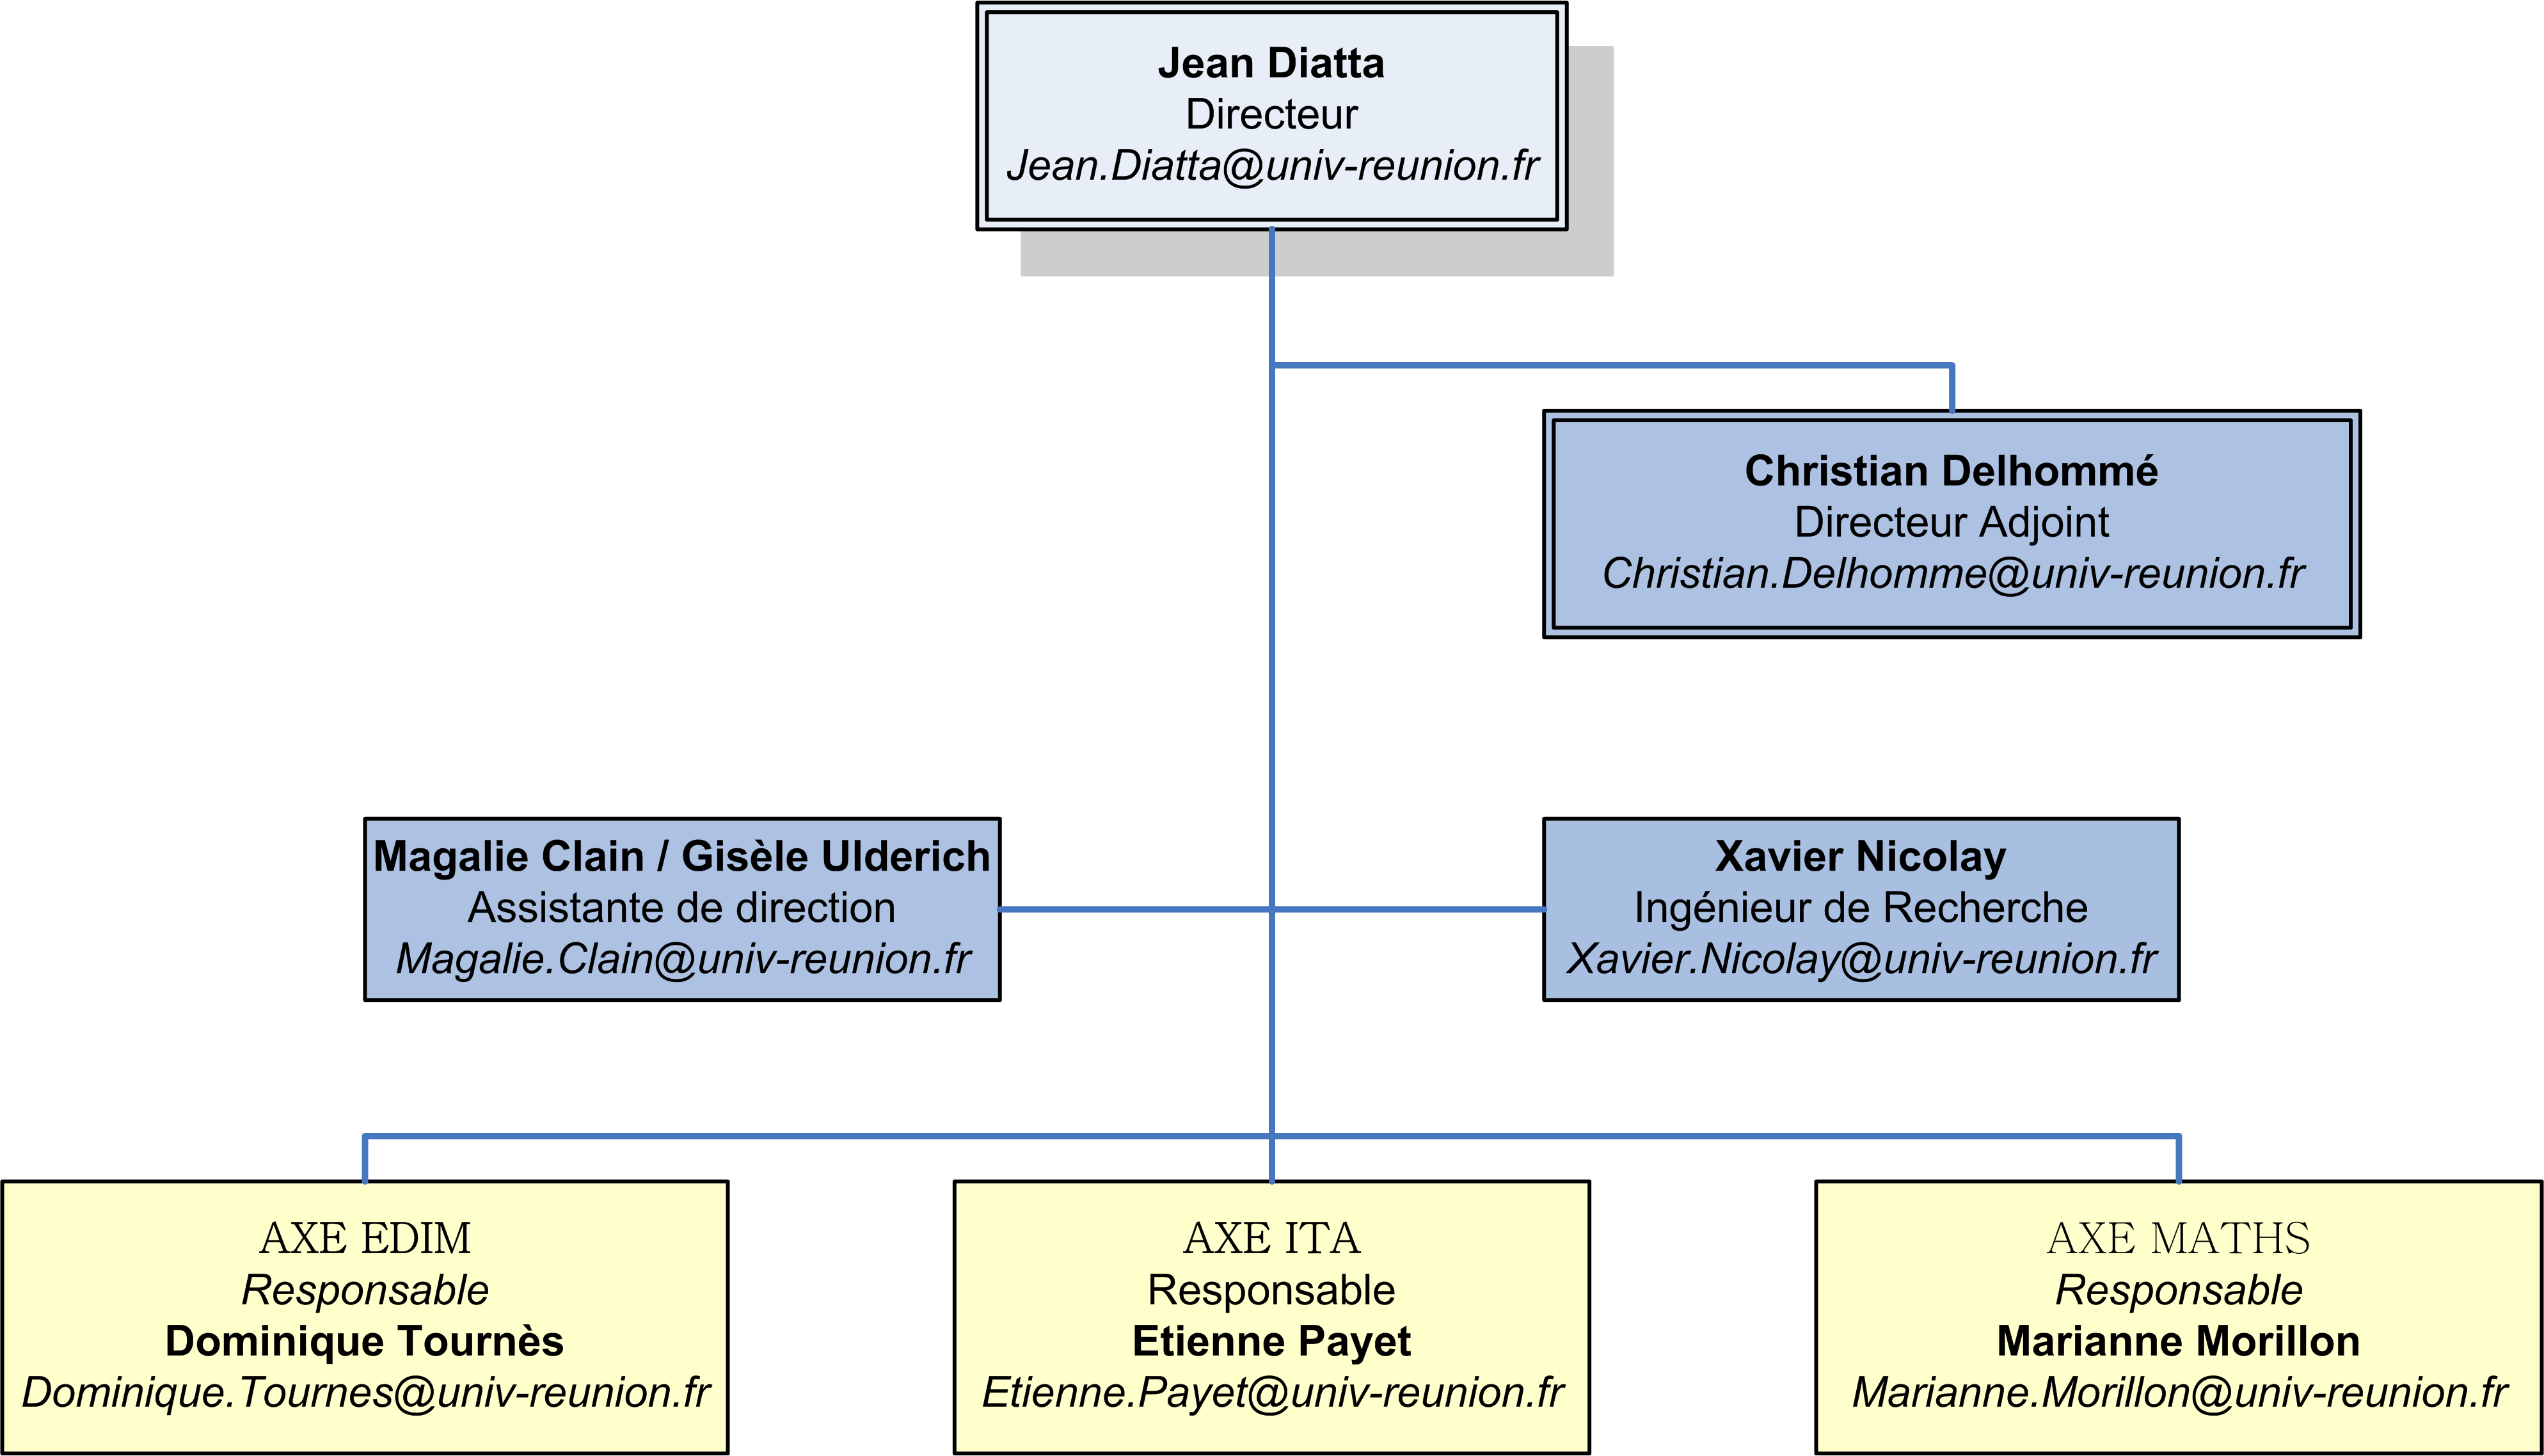
\includegraphics{OrganigrammeLIM-v3.png}
	\end{center}
\end{landscape}

\end{appendices}


